% AER E 361 Mission Report Template
% Spring 2023
% Template created by Yiqi Liang and Professor Matthew Nelson

% Document Configuration DO NOT CHANGE
\documentclass[12 pt]{article}
% --------------------LaTeX Packages---------------------------------
% The following are packages that are used in this report.
% DO NOT CHANGE ANY OF THE FOLLOWING OR YOUR REPORT WILL NOT COMPILE
% -------------------------------------------------------------------

\usepackage{hyperref}
\usepackage{parskip}
\usepackage{titlesec}
\usepackage{titling}
\usepackage{graphicx}
\usepackage{graphviz}
\usepackage[T1]{fontenc}
\usepackage{titlesec, blindtext, color} %for LessIsMore style
\usepackage{tcolorbox} %for references box
\usepackage[hmargin=1in,vmargin=1in]{geometry} % use 1 inch margins
\usepackage{float}
\usepackage{tikz}
\usepackage{svg} % Allows for SVG Vector graphics
\usepackage{textcomp, gensymb} %for degree symbol
\hypersetup{
	colorlinks=true,
	linkcolor=blue,
	urlcolor=cyan,
}
\usepackage{biblatex}
\addbibresource{lab-report-bib.bib}
\usepackage{amsmath}
\usepackage{listings}
\usepackage{multicol}
\usepackage{array}

\usepackage{hologo} %KYR: for \BibTeX
%\usepackage{algpseudocode}
%\usepackage{algorithm}
% This configures items for code listings in the document
\usepackage{xcolor}

\usepackage{fancyhdr} % Headers/Footers
\usepackage{siunitx} % SI units
\usepackage{csquotes} % Display Quote
\usepackage{microtype} % Better line breaks

\definecolor{commentsColor}{rgb}{0.497495, 0.497587, 0.497464}
\definecolor{keywordsColor}{rgb}{0.000000, 0.000000, 0.635294}
\definecolor{stringColor}{rgb}{0.558215, 0.000000, 0.135316}
\definecolor{mygreen}{rgb}{0,0.6,0}
\definecolor{mygray}{rgb}{0.5,0.5,0.5}
\definecolor{mymauve}{rgb}{0.58,0,0.82}

\lstdefinestyle{customc}{
  belowcaptionskip=1\baselineskip,
  breaklines=true,
  frame=L,
  xleftmargin=\parindent,
  language=C,
  showstringspaces=false,
  basicstyle=\footnotesize\ttfamily,
  keywordstyle=\bfseries\color{green!40!black},
  commentstyle=\itshape\color{purple!40!black},
  identifierstyle=\color{blue},
  stringstyle=\color{orange},
 }

 \lstset{ %
  backgroundcolor=\color{white},   % choose the background color; you must add \usepackage{color} or \usepackage{xcolor}
  basicstyle=\footnotesize,        % the size of the fonts that are used for the code
  breakatwhitespace=false,         % sets if automatic breaks should only happen at whitespace
  breaklines=true,                 % sets automatic line breaking
  captionpos=b,                    % sets the caption-position to bottom
  commentstyle=\color{commentsColor}\textit,    % comment style
  deletekeywords={...},            % if you want to delete keywords from the given language
  escapeinside={\%*}{*)},          % if you want to add LaTeX within your code
  extendedchars=true,              % lets you use non-ASCII characters; for 8-bits encodings only, does not work with UTF-8
  frame=tb,	                   	   % adds a frame around the code
  keepspaces=true,                 % keeps spaces in text, useful for keeping indentation of code (possibly needs columns=flexible)
  keywordstyle=\color{keywordsColor}\bfseries,       % keyword style
  language=Python,                 % the language of the code (can be overrided per snippet)
  otherkeywords={*,...},           % if you want to add more keywords to the set
  numbers=left,                    % where to put the line-numbers; possible values are (none, left, right)
  numbersep=8pt,                   % how far the line-numbers are from the code
  numberstyle=\tiny\color{commentsColor}, % the style that is used for the line-numbers
  rulecolor=\color{black},         % if not set, the frame-color may be changed on line-breaks within not-black text (e.g. comments (green here))
  showspaces=false,                % show spaces everywhere adding particular underscores; it overrides 'showstringspaces'
  showstringspaces=false,          % underline spaces within strings only
  showtabs=false,                  % show tabs within strings adding particular underscores
  stepnumber=1,                    % the step between two line-numbers. If it's 1, each line will be numbered
  stringstyle=\color{stringColor}, % string literal style
  tabsize=2,	                   % sets default tabsize to 2 spaces
  title=\lstname,                  % show the filename of files included with \lstinputlisting; also try caption instead of title
  columns=fixed                    % Using fixed column width (for e.g. nice alignment)
}

\lstdefinestyle{customasm}{
  belowcaptionskip=1\baselineskip,
  frame=L,
  xleftmargin=\parindent,
  language=[x86masm]Assembler,
  basicstyle=\footnotesize\ttfamily,
  commentstyle=\itshape\color{purple!40!black},
}

\lstset{escapechar=@,style=customc}

\titlelabel{\thetitle.\quad}

% From here on out you can start editing your document
\newcommand{\subtitle}[1]{%
  \posttitle{%
    \par\end{center}
    \begin{center}\LARGE#1\end{center}
    \vskip0.5em}%
}

\title{\textbf{Iowa State University
\\{\Large Aerospace Engineering}}}
\subtitle{AER E 322 Lab <lab number>\\
		  <lab name>}
\author{Matthew Mehrtens, Peter Mikolitis, and Natsuki Oda}

\newcommand{\etal}{\textit{et al}., }
\newcommand{\ie}{\textit{i}.\textit{e}., }
\newcommand{\eg}{\textit{e}.\textit{g}., }

% Define the headers and footers
\setlength{\headheight}{70.63135pt}
\geometry{head=70.63135pt, includehead=true, includefoot=true}
\pagestyle{fancy}
\fancyhead{}\fancyfoot{} % clears the headers/footers
\fancyhead[L]{\textbf{AER E 322}}
\fancyhead[C]{\textbf{Aerospace Structures Pre-Laboratory}\\
			  \textbf{Lab 03 Riveted Joint Design, Fabrication and Testing}\\
			  Section 4 Group 2\\
			  Matthew Mehrtens\\
			  \today}
\fancyhead[R]{\textbf{Spring 2023}}
\fancyfoot[C]{\thepage}

\begin{document}
\section*{Question 1} \label{question_1}
\textit{Review Week 4 lecture materials and MIL-R-47196A standard thoroughly.}

\section*{Question 2} \label{question_2}
\textit{(80 pts) A pre-specified design of 2-2 rivet pattern is given in Fig. 1 for a riveted sample consisting of two overlapped 2” by 8” test panels.  The thickness of each test panel is 0.025” and hole diameter (i.e. rivet diameter) is 1/8”.  Your first task of the prelab is to evaluate the test panel’s joint efficiency for each of the four failure modes as described in Week 4 lecture notes, particularly in the workout example on pages 18-28.  Which failure will happen first and why? Next, for each failure mode, predict the maximum load that can cause that type of failure.  For tension failure mode, calculate the maximum load and corresponding stress for each row separately, as demonstrated in Part 3 of the workout example.  Use the material properties provided below.}

Based on the output of my script shown in Listing \ref{code:rivet-analysis-2by2.m}, here are the predicted efficiencies:

\begin{align*}
\eta_s&=\num{0.6545} \\
\eta_b&=\num{0.463} \\
\eta_{to}&=\num{0.6667} \\
\eta_{t1}&=\num{0.875} \\
\eta_{t2}&=\num{1.75}
\end{align*}

Based on these efficiencies, bearing failure, $\eta_b$, will occur first since it has the lowest efficiency, \ie the system handles bearing loads the least efficiency.

The maximum loads that can cause each type of failure are listed below. These were also calculated using Listing \ref{code:rivet-analysis-2by2.m}.

\begin{align*}
F_s&=\qty{883.6}{lb} \\
F_b&=\qty{625}{lb} \\
F_{to}&=\qty{900}{lb} \\
F_{t1}&=\qty{1181}{lb} \\
F_{t2}&=\qty{590.6}{lb} \\
\sigma_{t1}&=\qty{27}{ksi} \\
\sigma_{t2}&=\qty{13.5}{ksi}
\end{align*}

Based on these data, the system will fail at \qty{625}{lb} due to bearing failure.

\section*{Question 3} \label{question_3}
\textit{(120 pts) Based on what you find in Section 2. above, redesign the joint for better strength within the same overlapped area.  You may want to consider popular rivet patterns such as 1-3-1 and 2-1-2 or higher density like 2-3-2 and 3-3-3.  You can use as many rivets as you like but remember that too many rivets can actually weaken the joint (remember the design rule of thumb on page 17 of lecture notes).  Calculate the joint efficiency and predict how and under what load your new design will fail in each failure mode, just like what you did in Section 2.  You don't necessarily need to follow the minimum pitch and edge margins specified in MIL-R-47196A, but if you do decide to disregard standard practice, you should justify why.  You will also need to be able to justify if you will take different approaches in redesigning the joint.}

Using the my Rivet Analysis script, Listing \ref{code:rivet-analysis-designed.m}, the best design I could come up with is a four by two pattern shown in Figure \ref{fig:my-design}.

\begin{figure}[!htbp]
\centering
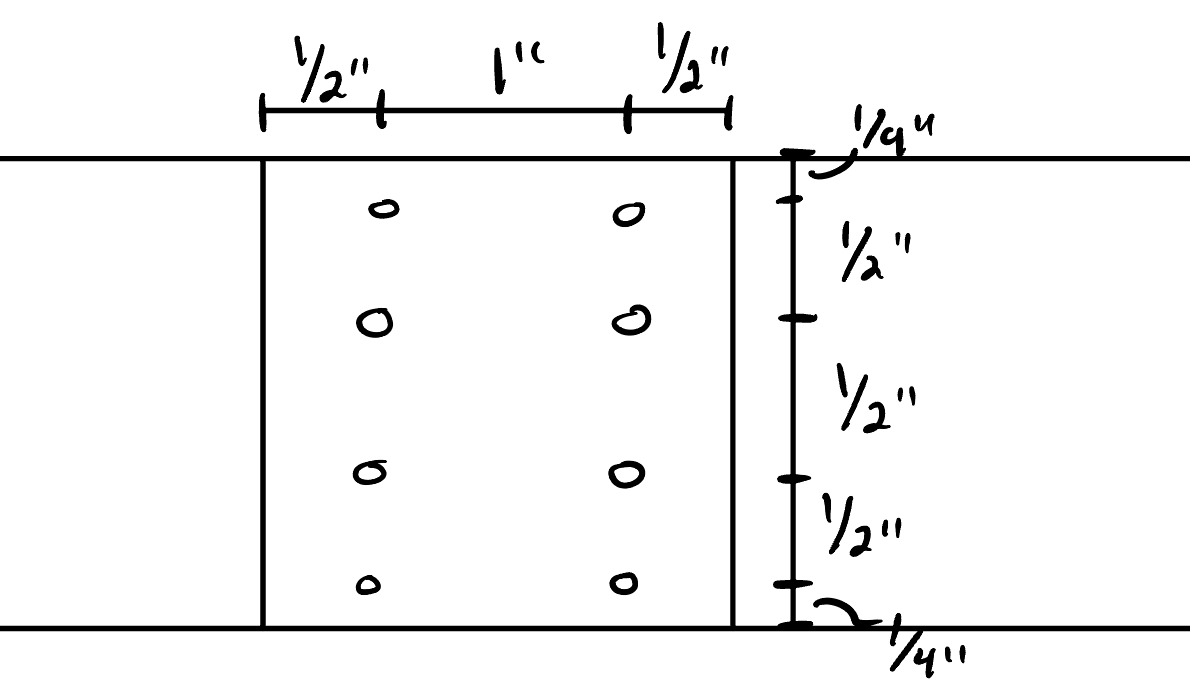
\includegraphics[width=4in]{images/my-design}
\caption{My rivet pattern design.}
\label{fig:my-design}
\end{figure}

The efficiencies are listed below:

\begin{align*}
\eta_s&=\num{1.309} \\
\eta_b&=\num{0.9259} \\
\eta_{to}&=\num{1.333} \\
\eta_{t1}&=\num{0.75} \\
\eta_{t2}&=\num{1.5}
\end{align*}

Based on these efficiencies, I expect my system to fail due to tension stress in the first row (relative to the loading) since it has the lowest efficiency of all the failure modes. The maximum loads supported by each mode of failure are:

\begin{align*}
F_s&=\qty{1767}{lb} \\
F_b&=\qty{1250}{lb} \\
F_{to}&=\qty{1800}{lb} \\
F_{t1}&=\qty{1012}{lb} \\
F_{t2}&=\qty{506.2}{lb} \\
\sigma_{t1}&=\qty{27}{ksi} \\
\sigma_{t2}&=\qty{13.5}{ksi}
\end{align*}

Given these maximum forces, I estimate my rivet pattern will be able to sustain a maximum of \qty{1012}{lb} before it fails due to tensile stress in the first row of rivets.

\section*{Code} \label{code}

\lstinputlisting[label={code:rivet-analysis-2by2.m},caption={Question 2 Script: \texttt{Rivet-Analysis-2by2.m}.},language=Matlab]{src/Rivet-Analysis-2by2.m}

\lstinputlisting[label={code:rivet-analysis-designed.m},caption={Question 3 Script: \texttt{Rivet-Analysis-Designed.m}.},language=Matlab]{src/Rivet-Analysis-Designed.m}

\lstinputlisting[label={code:calc-eta-shear.m},caption={Function to calculate $\eta_s$: \texttt{calc-eta-shear.m}.},language=Matlab]{src/calc-eta-shear.m}

\lstinputlisting[label={code:calc-eta-bearing.m},caption={Function to calculate $\eta_b$: \texttt{calc-eta-bearing.m}.},language=Matlab]{src/calc-eta-bearing.m}

\lstinputlisting[label={code:calc-eta-tearout.m},caption={Function to calculate $\eta_to$: \texttt{calc-eta-tearout.m}.},language=Matlab]{src/calc-eta-tearout.m}

\lstinputlisting[label={code:calc-eta-tension.m},caption={Function to calculate $\eta_t$: \texttt{calc-eta-tension.m}.},language=Matlab]{src/calc-eta-tension.m}

\end{document}
